\documentclass[border=5pt]{standalone}
\usepackage{pgfplots}
\pgfplotsset{compat=1.18}
\begin{document}
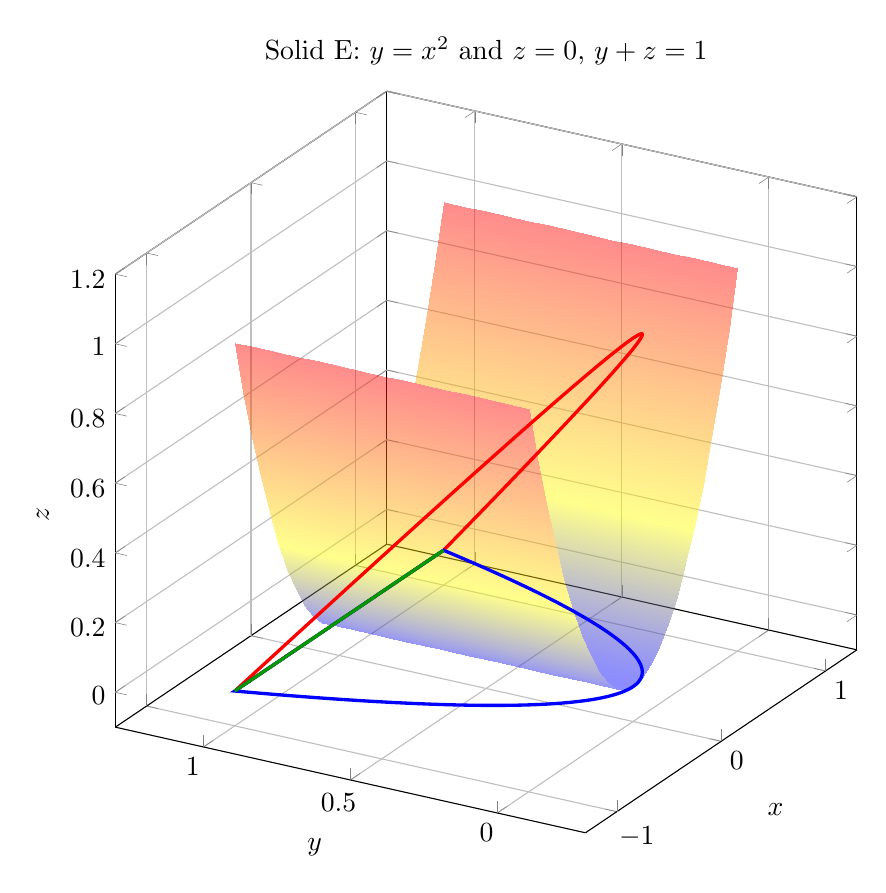
\begin{tikzpicture}
\begin{axis}[
    title={Solid E: $y=x^2$ and $z=0$, $y+z=1$},
    xlabel={$x$}, ylabel={$y$}, zlabel={$z$},
    view={-60}{25},
    xmin=-1.3, xmax=1.3,
    ymin=-0.3, ymax=1.3,
    zmin=-0.1, zmax=1.2,
    width=11cm, height=11cm,
    grid=major,
]

% Parabolic cylinder y = x^2 (orange)
\addplot3[
    surf, shader=interp,
    domain=-1:1, y domain=0:1,
    samples=25, samples y=15,
    opacity=0.45,
    color=orange,
] {x^2};

% Boundary curves
\addplot3[red, very thick, samples=80, domain=-1:1] (x, {x^2}, {1-x^2});
\addplot3[blue, very thick, samples=80, domain=-1:1] (x, {x^2}, 0);
\addplot3[green!60!black, very thick, samples=80, domain=-1:1] (x, 1, 0);

\end{axis}
\end{tikzpicture}
\end{document}